\section{Rancangan Solusi}
\label{sec:rancangan-solusi}

\subsection{Gambaran Umum}
Dengan segala kebutuhan yang sudah dianalisis, maka akan dibuat beberapa komponen penyusun sistem. Rencananya, sistem  akan dibuat menggunakan KubeEdge dan perangkat \textit{IoT} akan dibatasi jumlahnya sebanyak lima dan setiap perangkat akan diasumsikan sebagai \textit{cluster} yang berbeda.

\begin{figure}[h]
  \centering
  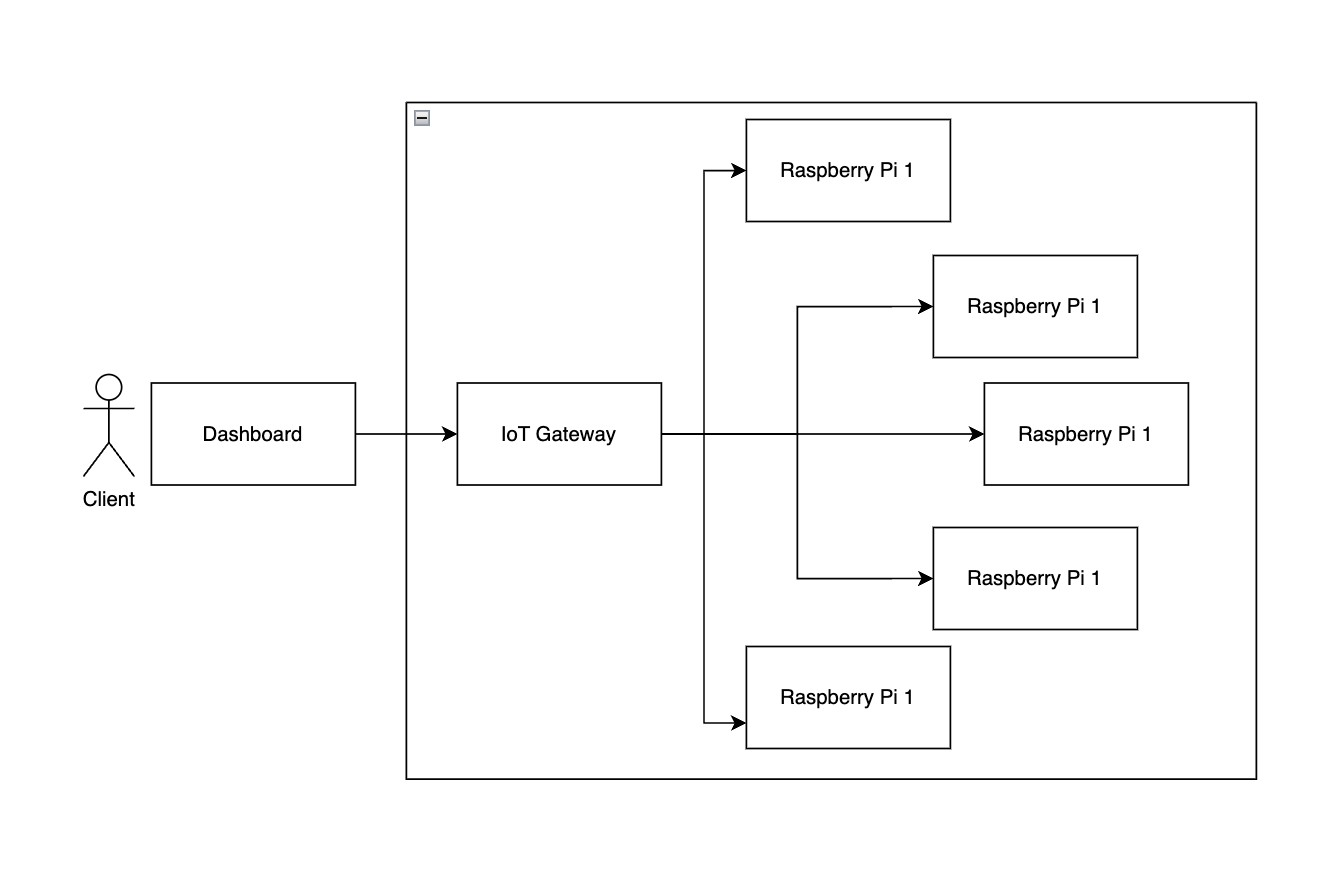
\includegraphics[width=0.5\textwidth]{resources/chapter-3/gambaran-umum-arsitektur.jpg}
  \caption{Gambaran umum arsitektur yang akan dibuat}
  \label{fig:gambaran-umum-arsitektur}
\end{figure}